% vim: set fdm=marker:
\pdfminorversion=4
\documentclass{beamer}

% theme {{{
%\usetheme{Antibes}
\usetheme[compress]{Dresden}
%\usecolortheme{dolphin}
\usecolortheme{rose}
%\usefonttheme{serif}
%}}}

% packages {{{
\usepackage[english]{babel}
\usepackage[utf8]{inputenc}
\usepackage[T1]{fontenc}
\usepackage{caption}
%}}}

% config {{{
\captionsetup{font=scriptsize,labelfont=scriptsize}
%}}}

% title {{{
\title{Analysis of Image Tranforms for Sketch-based Retrieval}
\subtitle{Diploma Thesis}
\author{Felix Stürmer}
\institute[Fakultät IV - TU Berlin]
{
    Technische Universität Berlin\\
    Fakultät IV - Elektrotechnik und Informatik\\
    Computer Graphics
}
\date{02.11.2012}
\subject{Computer Graphics}
%}}}

\begin{document}
% document {{{

% titlepage {{{
\begin{frame}
  \titlepage
\end{frame}
%}}}

% toc {{{
\begin{frame}{Outline}
  \tableofcontents
  % You might wish to add the option [pausesections]
\end{frame}
%}}}

% introduction and background {{{
\section{Introduction and Background}
\subsection{Motivation}
\begin{frame}{Motivation}
    foo
\end{frame}

\subsection{Challenges of CBIR}
\begin{frame}{Challenges of CBIR}
    \begin{block}{The Semantic Gap}
        \begin{quote}
            ``The semantic gap is the \textbf{lack of coincidence} between the
            information that one can extract from the \textbf{visual data} and
            the \textbf{interpretation} that the same data have for a user in a
            given situation.'' -- Smeulders et al.
        \end{quote}
    \end{block}
    \begin{block}{The Sensory Gap}
        \begin{quote}
            ``The sensory gap is the gap between the \textbf{object in the
            world} and the information in a (computational) description derived
            from a \textbf{recording of that scene}.'' -- Smeulders et al.
        \end{quote}
    \end{block}
\end{frame}

\subsection{Anatomy of a CBIR System}
\begin{frame}{Anatomy of a CBIR System}
    \begin{columns}
        \begin{column}{0.5\textwidth}
            \begin{figure}
                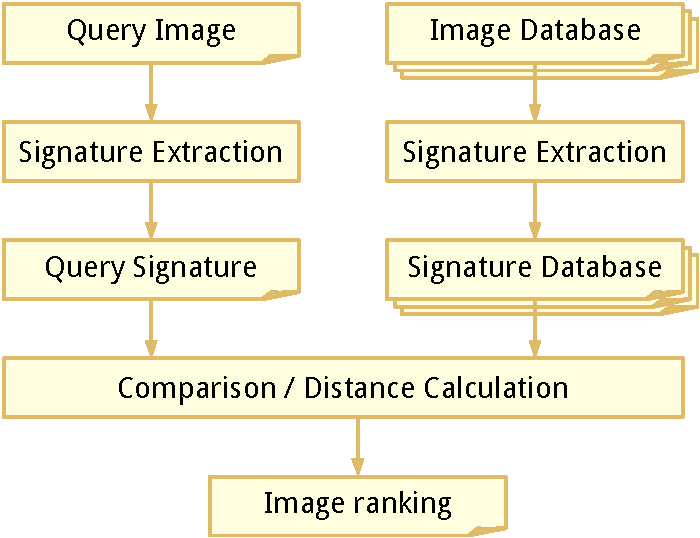
\includegraphics[width=.9\textwidth]{illustrations/cbir_anatomy_query_cropped}
                \caption{Global Descriptors}
                \label{fig:anatomy_global}
            \end{figure}
        \end{column}
        \begin{column}{0.5\textwidth}
            \begin{figure}
                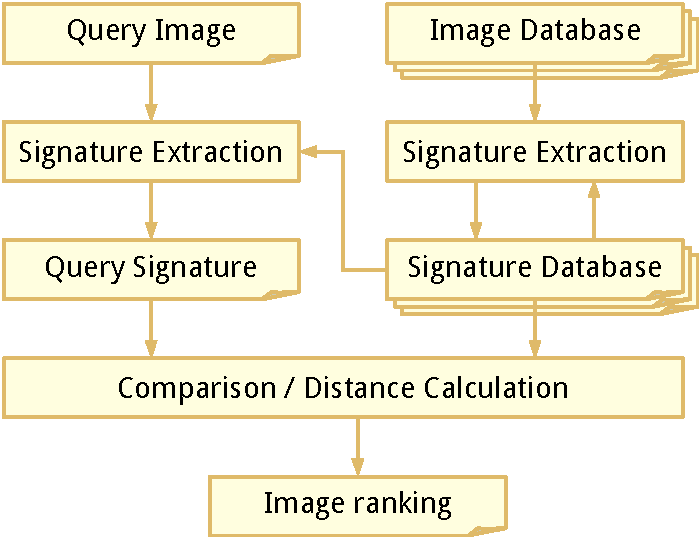
\includegraphics[width=.9\textwidth]{illustrations/cbir_anatomy_query_local_cropped}
                \caption{Local Descriptors}
                \label{fig:anatomy_local}
            \end{figure}
        \end{column}
    \end{columns}
\end{frame}
% }}}

% solution {{{
\section{Proposed Solution}
\subsection{Acquisition}
\begin{frame}{Acquisition}
    \begin{columns}
        \begin{column}{0.5\textwidth}
            \begin{figure}
                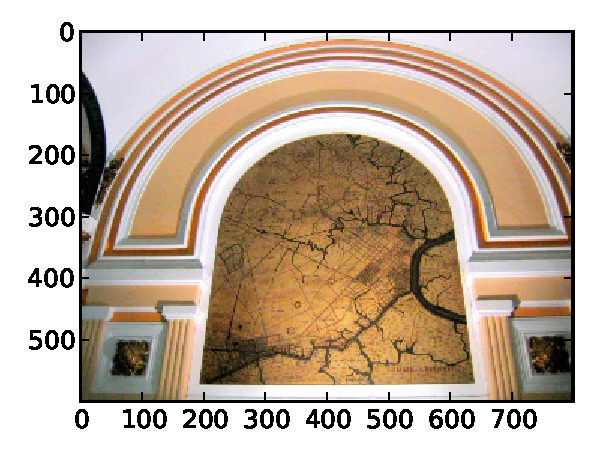
\includegraphics[width=\textwidth]{illustrations/input_example_color}
            \end{figure}
        \end{column}
        \begin{column}{0.25\textwidth}
            \begin{figure}
                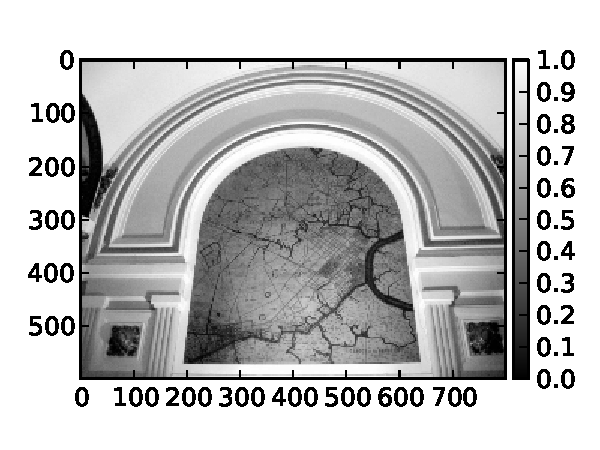
\includegraphics[width=\textwidth]{illustrations/input_example_luma}
                \caption{Luma Conversion}
            \end{figure}
            \begin{figure}
                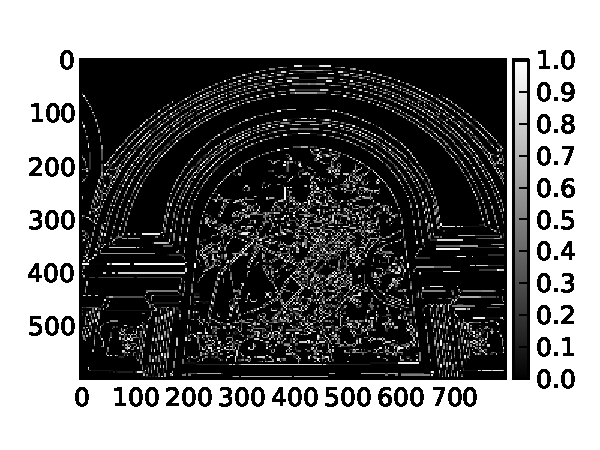
\includegraphics[width=\textwidth]{illustrations/input_example_canny}
                \caption{Canny Operator}
            \end{figure}
        \end{column}
        \begin{column}{0.25\textwidth}
            \begin{figure}
                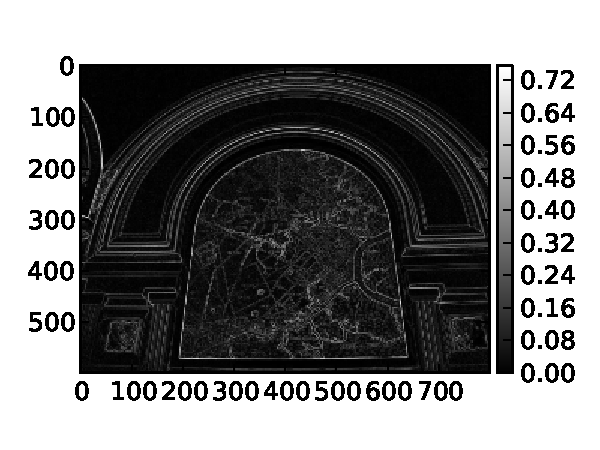
\includegraphics[width=\textwidth]{illustrations/input_example_sobel}
                \caption{Sobel Operator}
            \end{figure}
            \begin{figure}
                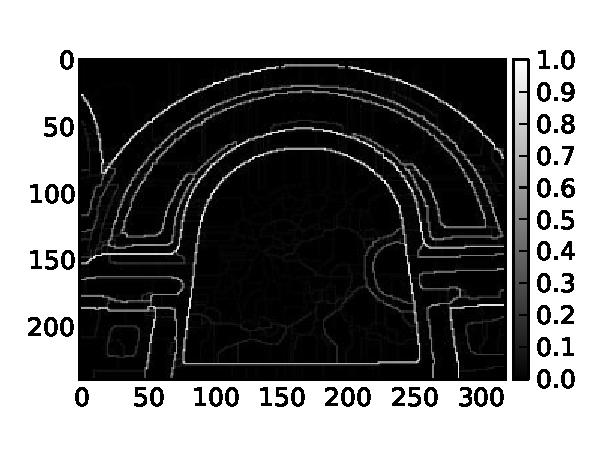
\includegraphics[width=\textwidth]{illustrations/input_example_segment}
                \caption{gPb-owt-ucm Transform}
            \end{figure}
        \end{column}
    \end{columns}
\end{frame}

\subsection{The Curvelet Transform}
\begin{frame}{The Curvelet Transform}
    foo
\end{frame}

\begin{frame}{The Fast Discrete Curvelet Transform}
    foo
\end{frame}

\subsection{Feature Extraction}
\begin{frame}{Global Feature Extraction}
    foo
\end{frame}

\begin{frame}{Local Feature Extraction}
    foo
\end{frame}

\subsection{Ranking}
\begin{frame}{Ranking}
    foo
\end{frame}
%}}}

% results {{{
\section{Results}
\subsection{Benchmarking}
\begin{frame}{Benchmarking Method}
    foo
\end{frame}

\subsection{Cross-Domain Results}
\begin{frame}{Cross-Domain Results}
    foo
\end{frame}

\subsection{Intra-Domain Results}
\begin{frame}{Intra-Domain Results}
    foo
\end{frame}
%}}}

% conclusion {{{
\section{Conclusions}
\begin{frame}{Conclusions}
    foo
\end{frame}
%}}}

%}}}
\end{document}
